{\color{gray}Consider the extendable hashing indexing mechanism introduced in the theoretical classes. Show how data records with the following keys can be stored in buckets which individually can hold 2 records, using extendable hashing and considering the least significant bits first in the directory of the resulting data structure.}

\textit{\color{gray}Azeitão, Camembert, Emmental, Serra , Camembert, Camembert, Creme, Alverca curado}

{\color{gray}Consider that binary representations for keys were determined by a simple hash function, resulting in:}


\begin{figure}[H]
	\begin{center}
	\begin{subfigure}[b]{0.5\textwidth}
		\centering
		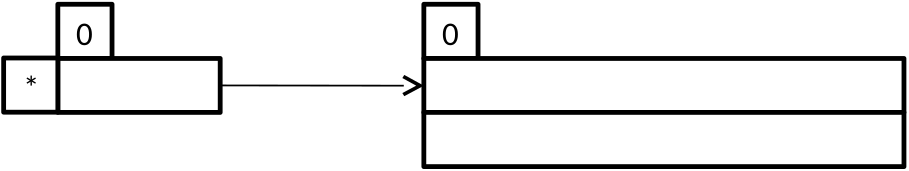
\includegraphics[width=\textwidth]{fig1.png}

	\end{subfigure}
	\caption{Estado inicial}
	\end{center}
\end{figure}
\begin{figure}[H]
	\begin{center}
	\begin{subfigure}[b]{0.5\textwidth}
		\centering
		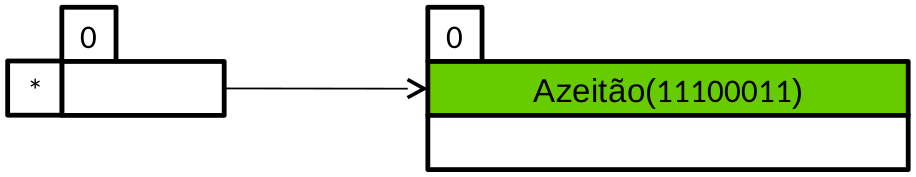
\includegraphics[width=\textwidth]{fig2.png}

	\end{subfigure}
	\caption{Azeitão - 11100011}
	\end{center}
\end{figure}
\begin{figure}[H]
	\begin{center}
	\begin{subfigure}[b]{0.5\textwidth}
		\centering
		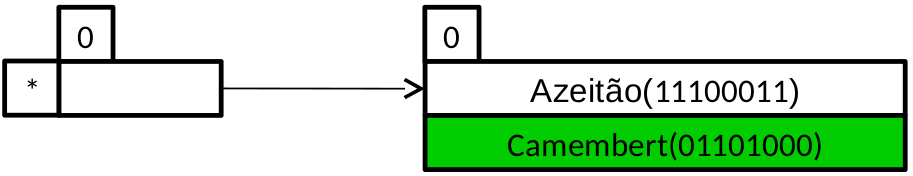
\includegraphics[width=\textwidth]{fig3.png}

	\end{subfigure}
	\caption{Camembert - 01101000}
	\end{center}
\end{figure}
\begin{figure}[H]
	\begin{center}
	\begin{subfigure}[b]{0.5\textwidth}
		\centering
		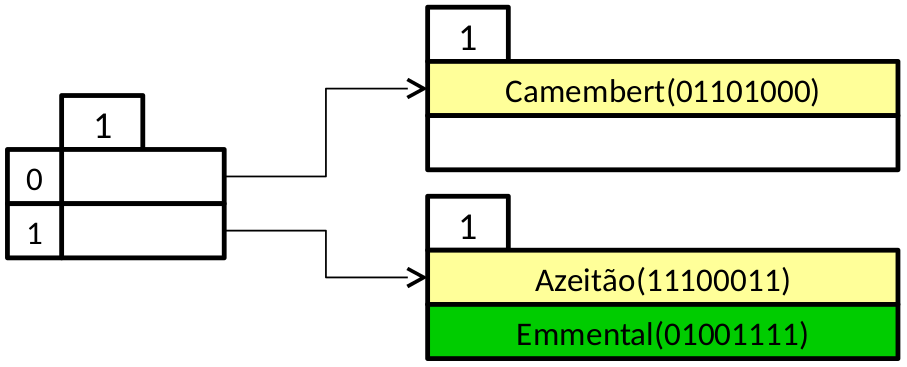
\includegraphics[width=\textwidth]{fig4.png}

	\end{subfigure}
	\caption{Emmental - 01001111}
	\end{center}
\end{figure}
\begin{figure}[H]
	\begin{center}
	\begin{subfigure}[b]{0.5\textwidth}
		\centering
		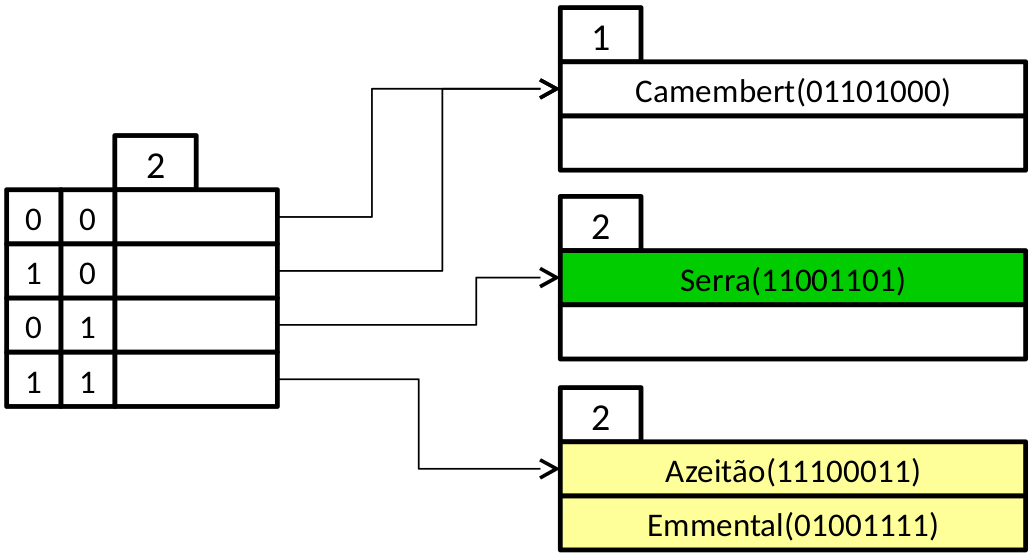
\includegraphics[width=\textwidth]{fig5.png}

	\end{subfigure}
	\caption{Serra - 11001101}
	\end{center}
\end{figure}
\begin{figure}[H]
	\begin{center}
	\begin{subfigure}[b]{0.5\textwidth}
		\centering
		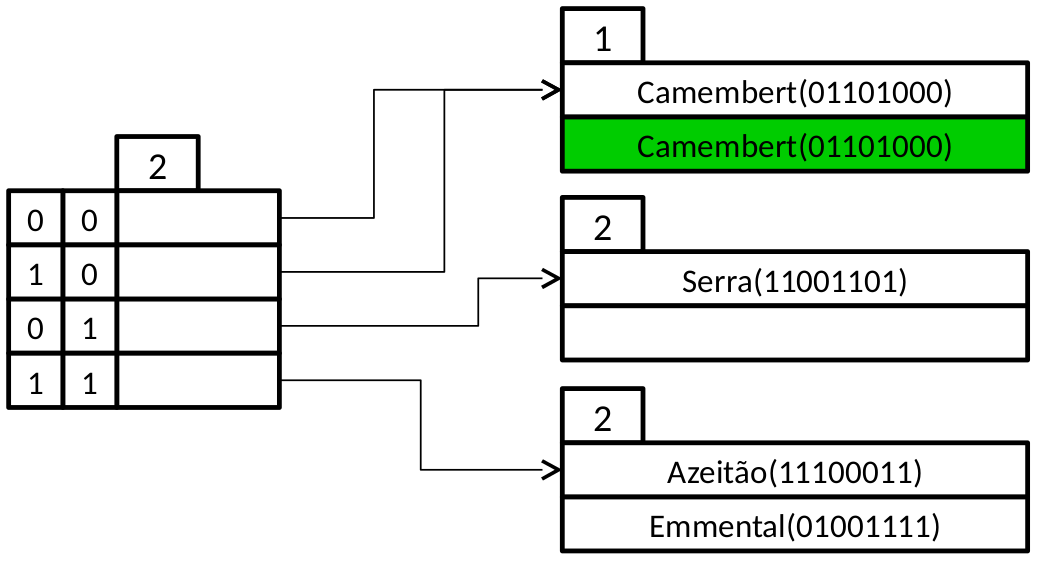
\includegraphics[width=\textwidth]{fig6.png}

	\end{subfigure}
	\caption{Camembert - 01101000}
	\end{center}
\end{figure}
\begin{figure}[H]
	\begin{center}
	\begin{subfigure}[b]{0.75\textwidth}
		\centering
		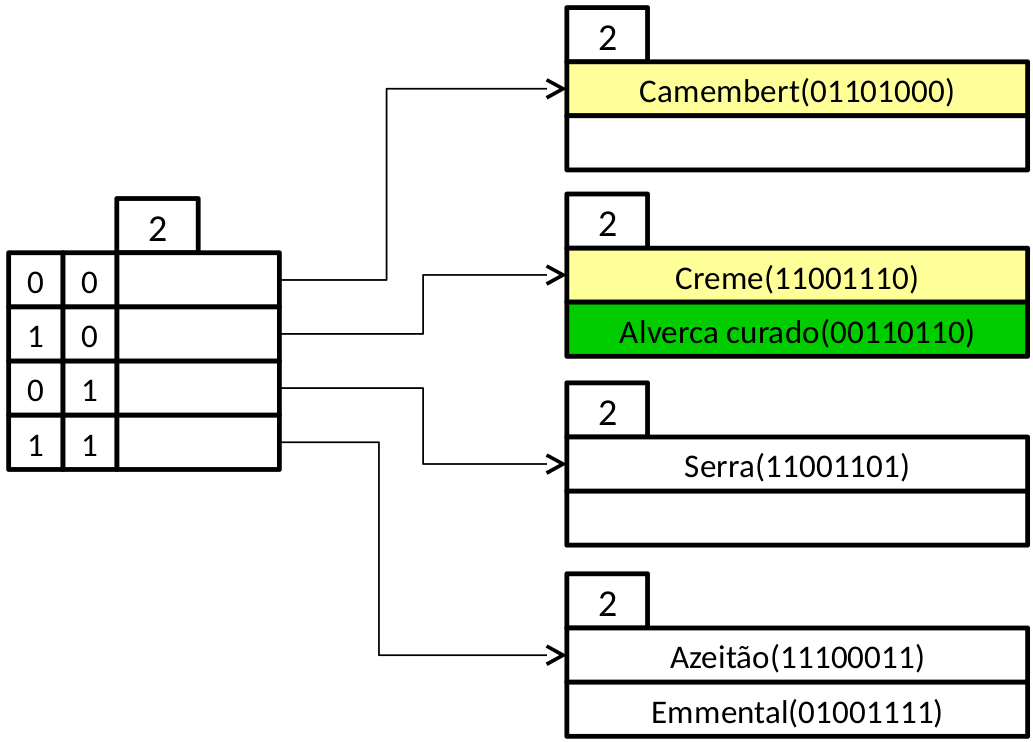
\includegraphics[width=\textwidth]{fig7.png}

	\end{subfigure}
	\caption{Camembert - 01101000}
	\end{center}
\end{figure}
\begin{figure}[H]
	\begin{center}
	\begin{subfigure}[b]{0.75\textwidth}
		\centering
		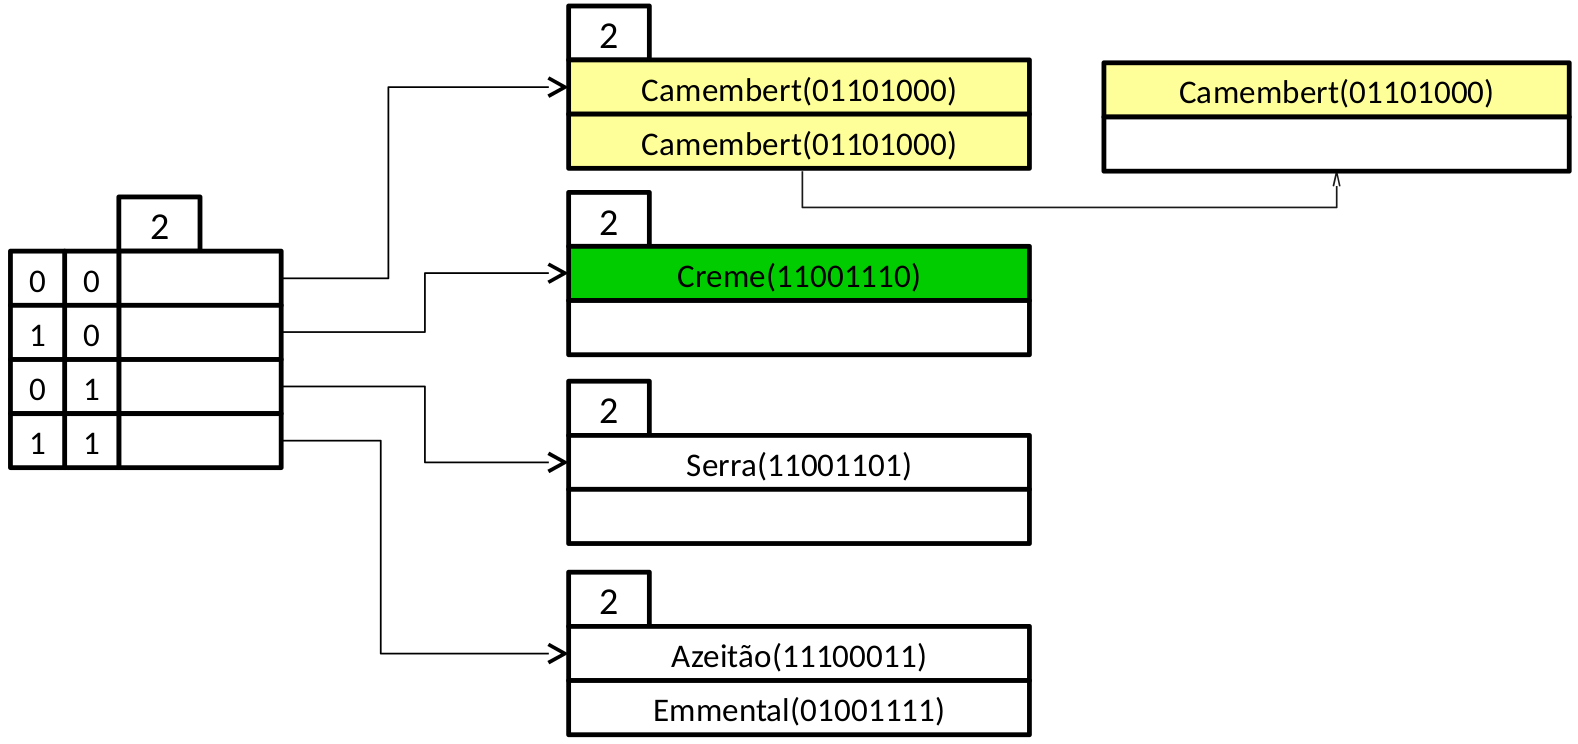
\includegraphics[width=\textwidth]{fig8.png}

	\end{subfigure}
	\caption{Creme - 11001110}
	\end{center}
\end{figure}
\begin{figure}[H]
	\begin{center}
	\begin{subfigure}[b]{0.75\textwidth}
		\centering
		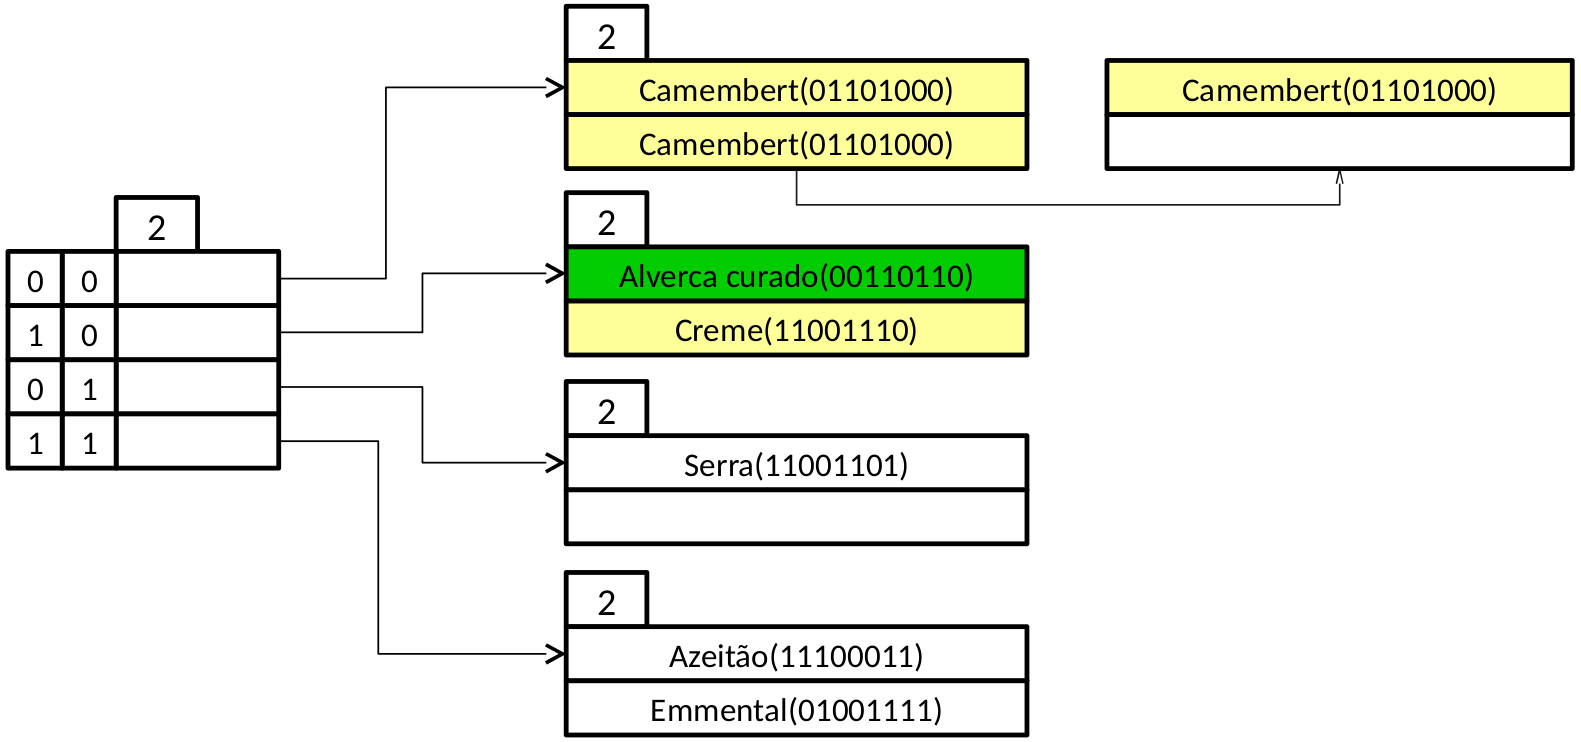
\includegraphics[width=\textwidth]{fig9.png}

	\end{subfigure}
	\caption{Alverca curado - 00110110}
	\end{center}
\end{figure}